\section{Введение}
\label{sec:Chapter0} \index{Chapter0}

В данной главе вводятся основные понятия, необходимые для постановки задачи.

\subsection{Файловая система}

Одна из основных функций операционной системы (ОС) - управление устройствами долговременного хранения информации и предоставление пользовательским приложениям интерфейса для взаимодействия с ними с целью хранения и организации доступа к данным. Элемент операционной системы, отвечающий за эти функции - \textbf{файловая система} (ФС). 

Для интеграции ряда файловых систем в единую структуру с пользовательской точки зрения в ядре ОС Linux используется концепция виртуальной файловой системы, позволяющая обращаться к различным файловым системам ипользуя единый интерфейс системных вызовов. Для оптимизации своей работы ФС использует множество внутренних структур данных. Для хранения метаданных пользовательских файлов и каталогов ФС использует структуру данных называемую \textbf{индексным дескриптором}. Также для хранения информации о свободном пространстве на устройстве файловые системы используют особые структуры данных, например битовую карту данных или список свободных блоков устройства. Для оптимизации процесса монтирования вся информация о файловой системе необходимая ОС в процессе монтирования хранится в структуре называемой \textbf{суперблоком}.

\subsection{Устройства долговременного хранения информации}

Большинство файловых систем ядра Linux были разработаны для взаимодействия с накопителями на жестком магнитном диске, особенности строения которых формировали алгоритмы хранения данных, используемые файловыми системами. Подобные устройства хранения состоят из вращающегося диска с магнитными дорожками и считывающей головки, способной перемещаться между дорожками. Из-за подобного строения доступ к произвольному блоку данных на жестком диске имел задержку позиционирования считывающей головки над нужной дорожкой и задержку вращения диска, обусловленную скоростью вращения магнитного диска. Для оптимизации задержки вращения в файловых системах использовались различные алгоритмы размещения данных на диске, например размещение файлов из одного каталога и их индексных дескрипторов поблизости.

С развитием технологий на рынке устройств долговременного хранения информации начали появляться аналоги жестким дискам в виде \textbf{устройств флеш-памяти}. Устройства флеш-памяти состоят из транзисторов, за счет чего скорость доступа к произвольному блоку имеет тот же порядок, что и скорость последовательного доступа к данным. Ячейки флэш-памяти организованы в так называемые \textbf{стираемые блоки}, которые обычно имеют размер 128 килобайт. Интерфейс взаимодействия с устройствами флэш-памяти отличается от интерфейса жесткого диска и составляет три основные команды: чтение данных из блока, стирание всего блока, то есть установка всех его бит в единицу и программирование памяти, то есть замена части единичных бит на нули для записи нужных данных, что может быть осуществлено после стирания блока.

Главная проблема флэш-памяти - износ. В процессе стирания и перезаписи блока на транзисторах накапливается избыточный заряд, из-за чего становится невозможно определить значение на транзисторе и блок становится непригодным к использованию. Время жизни блоков флэш-памяти измеряется в циклах стирания и имеет значение порядка 100000 циклов. Для предотвращения излишнего использования определенных блоков и продления срока службы всей микросхемы, используется технология \textbf{выравнивания износа} блоков, что означает равномерное использование всех блоков.

\subsection{Взаимодействие ФС с флэш-памятью}

Для эффективного использования флэш-памяти в качестве запоминающего устройства необходимо разрешить несколько основных проблем: выравнивание износа, обеспечение надежности в случае отключения питания, сборка мусора и необходимость програмной обработки дефектных блоков. Эти проблемы решаются \textbf{уровнем флэш-преобразования} (FTL). 

Уровень флэш-преобразования может быть размещен в контроллере устройства памяти, в драйвере устройства или в файловой системе, как это реализовано в JFFS2 и других ФС, взаимодействующих с неуправляемой флэш-памятью, например UBIFS и YAFFS2.

\subsection{Устройств на основе технологии памяти}

Для доступа к неуправляемой флэш-памяти, то есть не имеющей контроллера выполняющего функции FTL, в ядре Linux используется система устройств на основе \textbf{технологии памяти} (MTD - Memory Technology Device), предоставляющая базовые интерфесы для взаимодействия с устройствами, а также обработки и идентификации дефектных блоков. Структура подсистемы MTD проиллюстрирована на рис. ~\ref{mtd}.

\begin{figure}[H]
	\centering
	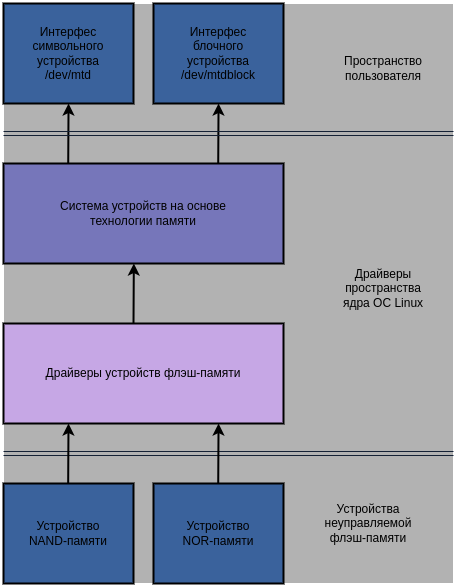
\includegraphics[scale=0.75]{mtd.png}
	\caption{Подсистема устройств технологии памяти (MTD)}
	\label{mtd}
\end{figure}

Она состоит из трех уровней: основной набор функций, драйверы микросхем флэш-памяти и драйверы пользовательского уровня, предоставляющие пользователю интерфейс символьного и блочного устройства для взаимодействия с флэш-памятью. 

\subsection{Файловая система JFFS2}

Файловая система JFFS2 (Journaling Flash Filesystem 2) была разработана для использования неуправляемых микросхем флэш-памяти в качестве запоминающего устройства и поддерживает устройства как NOR, так и NAND типа. JFFS2 является исторически первой файловой системой Linux для флэш-накопителей, но используется до сих пор. Она имеет журнальную структуру и использует подсистему устройств технологий памяти MTD для доступа к флэш-памяти.

Для того, чтобы избежать чтения всего журнала для вычисления структуры каталогов на этапе монтирования, JFFS2 использует сводные узлы (summary node). Сводный узел записывается в конец открытого стираемого блока и содержит в себе всю информацию, необходимую на этапе монтирования. Такой подход позволяет уменьшить время монтирования ценой небольшого перерасхода объема используемой памяти. Этот режим включается при установке определенного конфигурационного параметра ядра.

С целью различить является ли стираемый блок, в котором все биты установлены в 1 стертым, или он хранит полезную информацию, состояющую из всех единичных бит, JFFS2 использует маркеры очистки (clean marker), записываемые в начале блока. Если маркер очистки присутствует в блоке, значит блок очищен.

\subsection{Тестирования файловых систем}

Обеспечение надежности и отказоустойчивости модулей ядра, и файловой системы в частности - важная и непростая задача. Наличие ошибок в исходном коде ФС может привести к нарушениям в основных функциях файловой системы, получению пользователем несанкционированного доступа к привелигированному режиму ядра, а также полному краху или блокировке системы. Подобные последствия ошибок на серверах и суперкомпьютерах могут привести к потерям значимых данных или несанкционированному доступу к ним.

Большинство веб-серверов и суперкомпьютеров используют операционные системы на основе ядра Linux, имеющего открытый исходный код. В ядре Linux имеется множество файловых систем, разработанных для различных типов устройств хранения информации и использующие различные алгоритмы расположения данных на устройстве. 

Решением для проверки корректности функционирования операционных систем и их модулей является создание систем автоматизированного тестирования.  

Важнейшей метрикой, характеризующей качество подобных систем тестирования является тестовое покрытие кода. Полнота тестового покрытия кода является предметом для множества исследований, в том числе в области тестирования файловых систем. Данная работа посвящена созданию системы автоматизированного тестирования файловой системы JFFS2 и исследованию достигаемого тестового покрытия исходного кода этой файловой системы.

\newpage
